\section{Pali and Chinese Vinayas of the different schools}

\subsection{Theravāda Vinaya}
The {\em Theravāda Vinaya Khandhaka 1 Pabbajjā}\footnote{Pli-tv-kd 1 61} describes a {\em paṇḍaka} monk who is trying to have sex with monks and novices but is rebuked each time. He finally manages with the elephant and horse-keepers. The matter is brought to the Buddha who lays down a rule saying {\em paṇḍaka} cannot ordain and if they are already ordained they need to be expelled.

Further down there is the following passage\footnote{translation by Ajahn Brahmali}:

\begin{quote}
At one time an {\em ubhatob­yañ­janaka} had gone forth as a monk. He had sex and made others have it. They told the Buddha and he said, “An {\em ubhatob­yañ­janaka} should not be given the full ordination. If it has been given, he should be expelled.”
\end{quote}

Neither the {\em paṇḍaka} and the {\em ubhatob­yañ­janaka} are further defined here but the word {\em ubhatob­yañ­janaka} is a compound between {\em ubhato} meaning "in both ways, on both sides" and {\em byañjana} or {\em vyañjana} meaning "sign or mark".


\subsection{Mahāsaṅghika Vinaya}
The {\em Mahāsaṅghika Vinaya Bhikkhu Pakiṇṇaka} describes that monks feel groping at night and after catching the culprit, a monk, he admits being a 非男非女 i.e. neither male, nor female\footnote{T22n1425_023:0417c14–0418a10}. They report to the Buddha, who tells them there are six types of un-males (不能男 者有六種) (lit. those we are not capable of producing seed/impotent). The Buddha lays down a rule that none of these should be ordained and those already ordained should be expelled.

\begin{enumerate}
\item those born impotent (生). 
\item those who are born from a concubine (捺破)\footnote{This is the only place in the canon where this is mentioned but X44 0744_004 0432c13 mentions that there are 5 types of 黃門 (lit. yellow gate), which is translated as 'eunuch' elsewhere and 6 types of 種不能男 (i.e. seed incapable men), the 6th type being those born from a concubine}.
\item a castrated impotent man (割却), who is castrated as a punishment by the King's minister (割却 男根 lit. cut faculty of masculinity).
\item a transformed impotent man who is aroused by the touch of others but cannot ejaculate (因他)\footnote{This is a very free translation based on other texts where this type is mentioned}.
\item a jealous impotent man who is a voyeur and becomes aroused when watching others have sex (妬).
\item a 'half-moon' impotent man (半月生者) (description of what this is exactly is unclear).
\end{enumerate}

The term 非男非女 (neither male nor female) is only used by the {\em paṇḍaka} to describe himself in the this Vinaya. This could be a literal translation of the term {\em napuṃsaka} as in Vedic India this is an umbrella term of which the {\em paṇḍaka} is a subsection. The hijra of India also refer to themselves with this term.

The term 二根 (i.e. 2 roots/faculties) is mentioned in passing as a question for ordination but without further explanation. Also the term 黃門 (translated as 'eunuch') is also mentioned here without further explanation.


\subsection{Dharmaguptaka Vinaya}
In the {\em Dharmaguptaka Vinaya Pabbajja Khandhaka} the story is similar to that in the {\em Theravāda Vinaya}. A 'eunuch' (黃門) is ordained and then tries to have sex with monks and novices but is rebuked. He ends up having sex with cowherds and shepherds. The story is brought to the Buddha who lays down the rule that all 'eunuchs' have to be expelled and cannot ordain. He identifies five types of 'eunuchs'\footnote{translation by \cite{bodhi}. T22_1428 0812b23–0812c10}: 

\begin{enumerate}
\item those born as 'eunuch' (生黃門). 
\item a castrated 'eunuch' (犍黃門)\footnote{lit. a bullock-eunuch}.
\item a jealous 'eunuch' (妬黃門), who is aroused at the sight of others having sex.
\item a transformed 'eunuch' (變黃門). Transformed means while committing a sexual act with another, he loses masculine function, and thereby becomes a paṇḍaka.
\item a 'half-moon' 'eunuch' (半月黃門), having male function for half a month, and being impotent for the other half of the month\footnote{The word 不能男 (i.e. incapable/impotent) is used here just like in the Mahāsaṅghika Vinaya}.
\end{enumerate}

It is interesting to note that after the regular list of persons not to be ordained like animals, matricides, etc. the {\em Dharmaguptaka Vinaya} add here the story of a monk and nun resp. who change gender as is mentioned in the {\em Theravāda Pārājika 1}. The Buddha concludes that they can simply go to the other order and do not need to be expelled. The next paragraphs list the case of a monk and nun resp. who changed gender to become 男女二形 i.e. both male and female. The Buddha mentions that they have to be expelled but does not say that ordination is not possible for those who are already 男女二形 before. However we can conclude this by inference.

The {\em Dharmaguptaka Vinaya} proceeds to list details of monks who have been castrated through various causes. Obviously these are not seen as falling under the same category as the above mentioned 'eunuch'. Most of these, except for the one who self-castrates, can stay in robes; when castration happens through accident or even when it happens through karmic causes, the monk in question can remain, if he causes the castration intentionally himself he is expelled. Here the phrase is 截其 男根 (lit. cut off the male root).

While in the {\em Mahāsaṅghika Vinaya} the castration (i.e. cutting off of the male faculty 男根) is seen as an impotent man and thus not fit for ordination, here this only matters when the action is voluntary and not accidental.


\subsection{Mahīśāsaka Vinaya}
The story in the {\em Mahīśāsaka Vinaya Pabbajjā Khandhaka}\footnote{T22_1421 0117c29–0118a05} is similar to the {\em Theravāda Vinaya}. A {\em paṇḍaka} (黃門) is ordained and proceeds to try and have sex with various monks, novices and others. As a result that he is expelled together with others like him. Just like in the {\em Theravāda Vinaya}, there is no mention here of several types of {\em paṇḍaka}. At the end of the expulsion spoken by the Buddha, it is simply mentioned that the same holds true for 'two roots/faculties' (二根) without further explanation of what this is.

The story of the monk who became a woman and was allowed to live with the nuns thereafter is also mentioned here. The next paragraph is dedicated to a monk who, due to his great lust, self-castrated and as a result is expelled.


\subsection{Sarvāstivāda Vinaya}
The story in the {\em Sarvāstivāda Vinaya Pabbajjā Khandhaka}\footnote{T23_1435 0153b18–0153c17} also tells of a monk who groped other monks at night which gave problems and started rumours. Again, the Buddha identifies five types 種不能男 (impotent males). All these are not allowed to ordain and are expelled if already ordained.

\begin{enumerate}
\item those born impotent (生). (here possibly defined as a bastard)
\item a 'half-moon' impotent man (半月), who is impotent for half of the month.
\item a jealous impotent man (妬), who likes to see others engage in sex.
\item an 'essential'(?) impotent man (精), who causes others to have sex?
\item a ill impotent man who became impotent through illness (?) (病).
\end{enumerate}

In another part of the Vinaya this term 二根 (2 roots/faculties) is used next to the term 黃門 ('eunuch') but not in relation to ordination. {\em Pārājika} 1 (just like the {\em Pārājika} 1 of all the schools) mentions the existence of 4 kinds of offenders, men, women, 黃門 ('eunuch') and 二根 (2 roots/faculties). The same two words are used elsewhere in the {\em Sarvāstivāda Vinaya} while the word 種不能男 (impotent) is only used in the list for those who cannot ordain.


\subsection{Commentaries}

Going beyond the Vinaya itself into the commentarial scriptures, we find the following in the {\em Theravāda Mahāvagga-aṭṭhakathā} to explain more about the nature of these two classes. It defines five types of {\em paṇḍaka}\footnote{{\em Samantapāsādikā}: Vol. V, p. 1015f. Following translations/explanations as in \cite{bomhard}}:

\begin{enumerate}
\item {\em āsittapaṇḍaka}: a man who gains satisfaction from performing oral sex on another man and from swallowing his semen or who only becomes sexually aroused after swallowing another man’s semen. 
\item {\em usūyapaṇḍaka}: a voyeur, that is, a person who gains sexual satisfaction from watching others have sex. 
\item {\em opakkamikapaṇḍaka}: eunuch, due to castration.
\item {\em pakkhapaṇḍaka}: those who become sexually aroused in parallel with the phases of the moon\footnote{According to \cite{bomhard}, the term pakkhapaṇḍaka (Skt. {\em pakṣapaṇḍaka}) probably does not refer, as traditionally understood, to an individual who becomes sexually aroused parallel to the phases of the moon, i.e., to someone who is aroused during the fortnight of either the waxing or waning moon, but to someone “who acts wrongly sexually, who behaves badly sexually.” He hypothesizes that {\em pakkha} of the compound {\em pakkhapaṇḍaka} should be understood in terms of its alternative meaning “a cripple,” and that the corresponding Sanskrit should not be understood as {\em pakṣa} but rather {\em phakka} (“cripple,” adj. “lame, crippled, maimed”), derived from the Skt. verbal root {\em phakk}, (a) “to creep, to steal along; (b) to have a preconceived opinion; (c) to act wrongly, to behave badly.” He thus considers the third meaning of phakk as most relevant to the case at hand.}.
\item {\em napuṁsakapaṇḍaka}: a person born without sexual organs. 
\end{enumerate}

It is interesting to note that here not all {\em paṇḍaka} are barred from ordination, in contrast to what the Vinaya mentions. Only the last three types are forbidden to ordain\footnote{\cite{wong} and \cite{thanissaro}}.

For the {\em ubhatob­yañ­janaka} we find the following\footnote{translation by Ajahn Brahmali}:

\begin{quote}
Because of kamma giving rise to female characteristics and kamma giving rise to male characteristics, there is for them the characteristics of both. With the male characteristic they act to transgress through sexual intercourse with women. Having encouraged another, they cause action in their own female characteristic. 

They are twofold: the female {\em ubhatob­yañ­janaka} and the male {\em ubhatob­yañ­janaka}. In regard to this, the female characteristic of the female {\em ubhatob­yañ­janaka} is apparent, but the male characteristic is hidden. The male characteristic of the male {\em ubhatob­yañ­janaka} is apparent, but the female characteristic is hidden. 

While the female {\em ubhatob­yañ­janaka} is acting with manliness among women, the female characteristic is hidden, whereas the male characteristic is apparent. 
When the male {\em ubhatob­yañ­janaka} enters the state of a woman for the sake of men, the male characteristic is hidden, whereas the female characteristic is apparent. 
The female {\em ubhatob­yañ­janaka} becomes pregnant and causes others to become pregnant. The male {\em ubhatob­yañ­janaka} does not become pregnant, but causes others to become pregnant. This is the difference between them."
\end{quote}

The Chinese equivalent of the {\em Samantapāsādikā} can be found in T24 1462: 善見律毘婆沙\footnote{T24n1462:0792c03–0792c06. 5th century CE. See also \href{https://zh.wikipedia.org/zh-hk/%E5%96%84%E8%A6%8B%E5%BE%8B%E6%AF%98%E5%A9%86%E6%B2%99}{Wikipedia}}:
\begin{quote}
There are three kinds of 2-facultied people (二根): those who can impregnate and conceive; those who can impregnate but not conceive; and those who cannot impregnate but who can conceive. These three types of people are not allowed to become monks and take the full precepts; if they have already taken the full precepts, they should be expelled.
\end{quote}

Other Chinese commentaries have variations of he same passage. For instance Shinsan X44 0744 0450b01–0450b04 mentions:
\begin{quote}
It is said that a person has two roots/faculties (二根): male and female. There are three kinds: The first is able to self-reproduce. He can impregnate and conceive. The second can impregnate others but cannot conceive himself. The third type cannot impregnate but he can conceive when impregnated by another. 
\end{quote}

\subsection{Summary}
The first thing that is striking when comparing the various Chinese schools is that there is no clear consistent term that denotes the {\em paṇḍaka}. The {\em Mahāsaṅghika and Sarvāstivāda} use the term 種不能男 (impotent lit. incapable of producing seed) in the descriptions in the first Khandhaka on ordination. In the {\em Dharmaguptaka}, this term is only used in the description of the 'half-moon' {\em paṇḍaka}. The term 黃門 (eunuch) is used in the {\em Dharmaguptaka and Mahīśāsaka Vinaya} while in the Sarvāstivāda Vinaya uses the term everywhere but in the ordination Khandhaka. As both the terms 種不能男 (impotent) and 黃門 (eunuch) are used in the same way in different schools, we can assume that both can denote {\em paṇḍaka} but that the difference in terms point to historical changes in understanding and translation\footnote{Shinsan text X44 0744_004 0432c13 (四分律名義標釋 第4卷) links both terms, see above.}.

The translation 'eunuch' is a later interpolation due to the etymological development of the Chinese 黃門, meaning 'yellow gate' and derived from the palace eunuchs in the Early Han Dynasty,\footnote{The word 黃門 is translated as 'eunuch' but the characters spell a different word, namely 'yellow gate'. The etymology of the word can be traced back to the Han Dynasty. See Shinsan text X44 0744_004 0432c09–0433a01: 此翻黃門。阿毗曇。譯為閹人。以無男根故。"This is a 黃門. Translated as castrated man. Because he has no male roots/faculty." This tells the story of the imperial ruler who appointed eunuchs to work for him. Yellow is the color of the middle in the "Five Directions" and of the earth in the "Five Elements" and therefore stands for imperial power and state. The color is only used by the emperor and others are not allowed to wear it. Therefore, the palace of the emperor is called the "Yellow Gate". In the Easter Han Dynasty, the emperor hired eunuchs and they held rather powerful positions as palace guards, scribes and other official functions. They were called the "yellow gates". It is a long story but the eunuchs became very powerful and eventually caused the downfall of the Han Dynasty (see \href{https://en.wikipedia.org/wiki/Han_dynasty}{Wikipedia}). So "yellow gate" became a synonym for 'eunuch'.} while the word 'impotent' seems to be an earlier interpretation and we also find this back in in the Vedic scriptures\footnote{see \cite{zwilling}}. The Chinese culture was vastly different from the Indian culture and I suspect that their own palace eunuchs were the only thing they could relate to as an explanation of the term {\em paṇḍaka}.

The following table compares the description of the various schools, adding the Sanskrit\footnote{Abhidharmakośavyākhyā-Skt: 94, 15–25} and Tibetan\footnote{Abhidharmakośavyākhyā-Tib: D, vol. gu, 85b6–86a3; P, vol. cu, 97b2–7} for reference\footnote{See \href{http://www.itlr.net/hwid:281142}{itlr.net} for details as well a more complete listing of possible meanings and occurrences of these terms}.

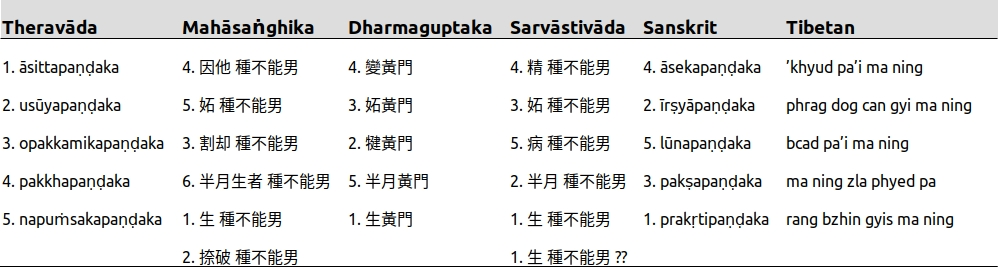
\includegraphics[width=\linewidth]{pandaka.jpg}
\captionof{figure}{Types of {\em paṇḍaka} in the various Buddhist schools}
\label{pandaka}

It is striking that the {\em Dharmaguptaka Vinaya} continues to describe several types of castrated men but does not equate these to {\em paṇḍaka}, while the word used for {\em paṇḍaka} is 黃門 (i.e. eunuch), which is the exact definition of a castrated man.

The {\em Theravāda and Mahīśāsaka Vinaya} agree on both the background story and do not mentioning a list of types of {\em paṇḍaka}, but the five types of {\em paṇḍaka} are described in the commentaries. The other Vinayas all have a list of {\em paṇḍaka} who are not allowed to ordain but some of these types differ from each other or seem to have a different description.

It is possible that at the time when the five types of {\em paṇḍaka} were introduced, the {\em Theravāda and Mahīśāsaka Vinaya} were already considered closed and therefore these five types appear in the commentarial text instead\footnote{Although the {\em Samantapāsādikā} is attributed to Buddhaghosa in the 5th century CE, this was based on earlier ones, now lost, in Prakrit and Sinhala, which were written down at the same time as the Canon, in the last century BCE. As we see here, some material in the commentaries is found in canonical texts of other schools, suggesting an early common source.}. 

The {\em Śāriputraparipṛcchā} attributes the schism of the {\em Mahāsaṅghika} school with the other schools at around 150 BCE to an attempt to expand the Vinaya by the other schools\footnote{See \cite{sujato2012}}. I therefore believe that the inclusion of the five types of {\em paṇḍaka} happened before this schism but was not originally in the Vinaya.

The fact that the descriptions of the five terms do not always seem to match seamlessly between schools and that there is some confusion over the term 'impotent', seemingly also denoting those who are socially impaired from marriage (i.e. the concubine's son) as well as the different description of a castrated man in both the {\em Dharmaguptaka and Mahīśāsaka Vinaya} seem to point to some ambiguity as to the meaning of {\em paṇḍaka} and the inclusion of the five types could have been an attempt to resolve this.

Considering that the word {\em paṇḍaka} does not appear in any of the early suttas\footnote{\cite{vimala}}, it seems clear that the inclusion of the word in the Vinaya did not happen in the Buddha's lifetime but was added later, possibly as a result of the discussions with the Brahmins and Jains, for whom the {\em paṇḍaka} could not ordain.
